\subsection{Tarefa 03}

\begin{comandoquestao}
Objetivo. Investigar como diferentes taxas de aprendizado 
(\texttt{learning\_rate}) afetam a 
convergência e o desempenho da rede neural. Analisaremos como a velocidade e a 
estabilidade do treinamento variam com a alteração dessa taxa.
\end{comandoquestao}

Nessa atividade treinamos uma mesma rede neural com os mesmos dados de testes, 
variando apenas a taxa de aprendizado ($\alpha$) e verificando o seu 
comportamento durante 
o treinamento e a capacidade de previsão da rede. Treinamos as redes para 
$\alpha = 0,001 | 0,01 | 0,05 | 0,1$. A evolução do erro durante o treinamento 
para as redes é mostrada na \cref{tarefa03:tabela:curvas}. As 
capacidades de previsão das redes são mostradas nas figuras 

\begin{figure}[tbh]
	\centering
	\caption{Curvas de perda durante treinamento (modificando $\alpha$)}
	\label{tarefa03:tabela:curvas}
	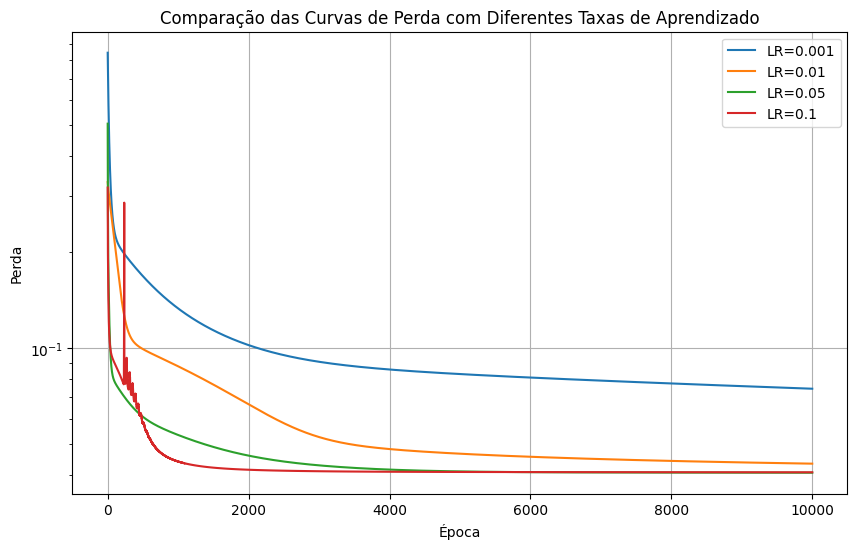
\includegraphics[width=0.7\linewidth]{./0803_imgs/png-241110-180530307-18269409044321663699.png}
\end{figure}


\begin{figure}[htb]
	\centering
	\begin{minipage}{0.45\textwidth}
		\centering
		\caption{$\alpha = 0,001$}\label{tarefa03:0001:predicoes}
		
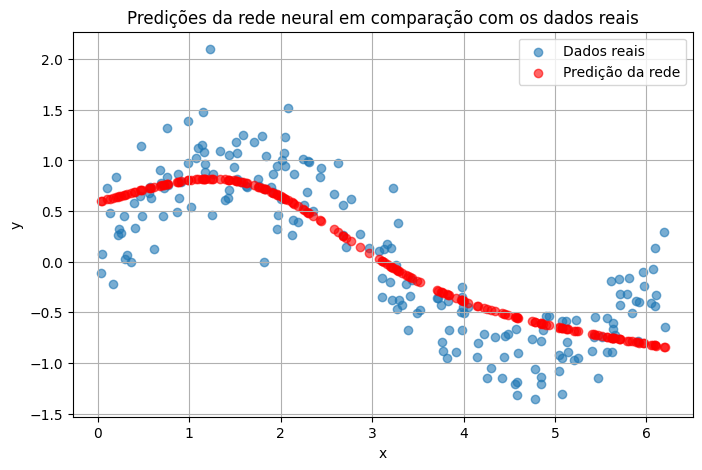
\includegraphics[width=\textwidth]{./0803_imgs/png-241110-175032242-2586281422306343440.png}
		%\legend{Fonte: Gerado peloComando da atividade}
	\end{minipage}
	\hfill
	\begin{minipage}{0.45\textwidth}
		\centering
		\caption{$\alpha = 0,01$}\label{tarefa03:001:predicoes}
		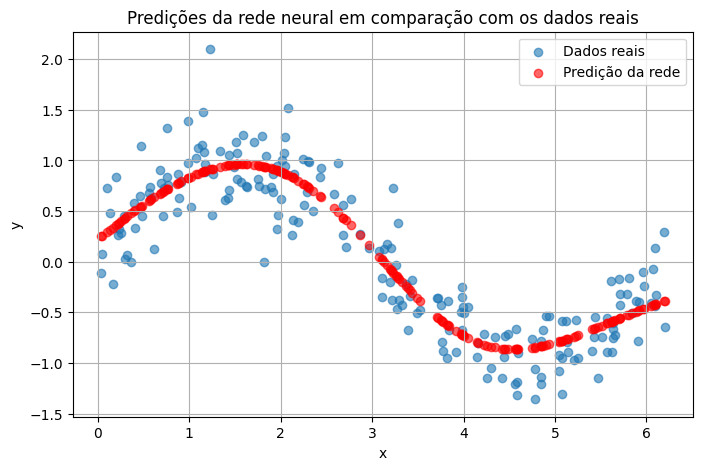
\includegraphics[width=\textwidth]{./0803_imgs/png-241110-175254024-1064294634935646228.png}
		%\legend{Fonte: \citeonline[p. 24]{araujo2012}}
	\end{minipage}
%	\vspace{1Ex}
%	\begin{minipage}{0.45\textwidth}
%		\centering
%		\caption{{$\alpha = 0,05$}\label{tarefa03:005:predicoes}
%		%\includegraphics[width=\textwidth]{./0803_imgs/}
%		%\legend{Fonte: \citeonline[p. 24]{araujo2012}}
%	\end{minipage}
%	\hfill
%	\begin{minipage}{0.45\textwidth}
%		\centering
%		\caption{{$\alpha = 0,1$}\label{tarefa03:01:predicoes}
%		%\includegraphics[width=\textwidth]{./0803_imgs/}
%		%\legend{Fonte: \citeonline[p. 24]{araujo2012}}
%	\end{minipage}
\end{figure}